\documentclass[times, twoside]{zHenriquesLab-StyleBioRxiv}
\usepackage{blindtext}
\usepackage[utf8]{inputenc}
\usepackage{graphicx}

\DeclareMathOperator*{\E}{\mathbb{E}}
\newcommand{\norm}[1]{\left\lVert #1 \right\rVert}

% Please give the surname of the lead author for the running footer
\leadauthor{Denovellis} 

\begin{document}

\title{A state space model for discovering the trajectory dynamics of replay}
\shorttitle{Replay Dynamics}

% Use letters for affiliations, numbers to show equal authorship (if applicable) and to indicate the corresponding author
\author[4]{Eric L. Denovellis}
\author[2, 3]{Anna K. Gillespie}
\author[2, 3]{Michael E. Coulter}
\author[1]{Uri T. Eden}
\author[2, 3, 4, \Letter]{Loren M. Frank}


\affil[1]{Department of Mathematics and Statistics, Boston University, Boston, Massachusetts}
\affil[2]{Department of Physiology, University of California, San Francisco, San Francisco, California}
\affil[3]{Kavli Institute for Fundamental Neuroscience, University of California, San Francisco, San Francisco, California}
\affil[4]{Howard Hughes Medical Institute, University of California, San Francisco, San Francisco, California}

\maketitle

%TC:break Abstract
%the command above serves to have a word count for the abstract
\begin{abstract}
During sleep and immobility, hippocampal place cells fire in sequences consistent with temporally compressed versions of trajectories previously run by the animal. These replayed sequences are hypothesized to be an important mechanism for the retrieval of spatial memory in service of consolidation and decision-making. Replay events are typically evaluated based on whether they activate sequences of place cells that represent spatially continuous trajectories through the environment, but recent work has shown that these events can have more complex dynamics. For example, sequences can alternate between hovering on a particular spatial location and continuous movement or can represent continuous trajectories in other spatial environments, which may appear spatially incoherent in the context of the current environment.

To quantify the structure of replay events, we develop a state space model that uses a combination of discrete and continuous latent state to decompose place cell sequences into categories based on their latent dynamics. Each discrete latent “category” is associated with a type of continuous latent dynamic—hovering in place, spatially fragmented or spatially continuous. This allows for (1) direct comparison between different categories of sequence dynamics, (2) expression of our confidence in one or more categories explaining the data, and (3) characterization of the transitions between categories. In addition, the model can function in 2D, avoiding linearization errors on more complicated environments. We demonstrate the utility of this model on simulated and real data of an animal performing a spatial memory task.

\end {abstract}
%TC:break main
%the command above serves to have a word count for the abstract

\begin{keywords}
Hippocampus | Replay | State Space
\end{keywords}

\begin{corrauthor}
%\texttt{loren{@}phy.ucsf.edu}
loren\at phy.ucsf.edu
\end{corrauthor}

\section*{Introduction}
The hippocampus is a brain area that is important for short term learning and memory. Neurons in the hippocampus preferentially fire in response to specific locations in an environment, which results in sequences of cells firing as an animal moves through an environment that reflect the trajectory of the animal. When the animal is asleep or immobile, cells also fire in sequence, forming trajectory-like representations that can recapitulate sequences previously observed when the animal was running. These sequences are thought to be important for memory consolidation or prospective decision making. (cite some examples). Therefore, characterizing the dynamics of hippocampal sequences is important for understanding memory consolidation and prospective decision making.

Current methods analyze hippocampal sequences by assuming a constant velocity trajectory \cite{DavidsonHippocampalReplayExtended2009}, corresponding to a single dynamic. This is done by computing the probability of position at each time using the place field information from the population of neurons and then fitting a line to maximize the probability of position over time. If the probabilities near the best fit line are high relative to shuffled distribution, the replay is analyzed. Often, trajectories that travel less than a certain distance \cite{PfeifferAutoassociativedynamicsgeneration2015} are excluded.

However, there is a growing evidence that trajectories that have more complex dynamics. Farooq and Dragoi \cite{FarooqEmergencepreconfiguredplastic2019} found that juvenile rats . For example, Pfeiffer and Foster \cite{PfeifferAutoassociativedynamicsgeneration2015} found that trajectories alternated between stationary hovering trajectories and continuous movement trajectories on a gamma timescale. 

Our mathematical model precisely specifies the dyna

\section*{Results}
\subsection*{Test}

\begin{figure*}%[tbhp]
\centering
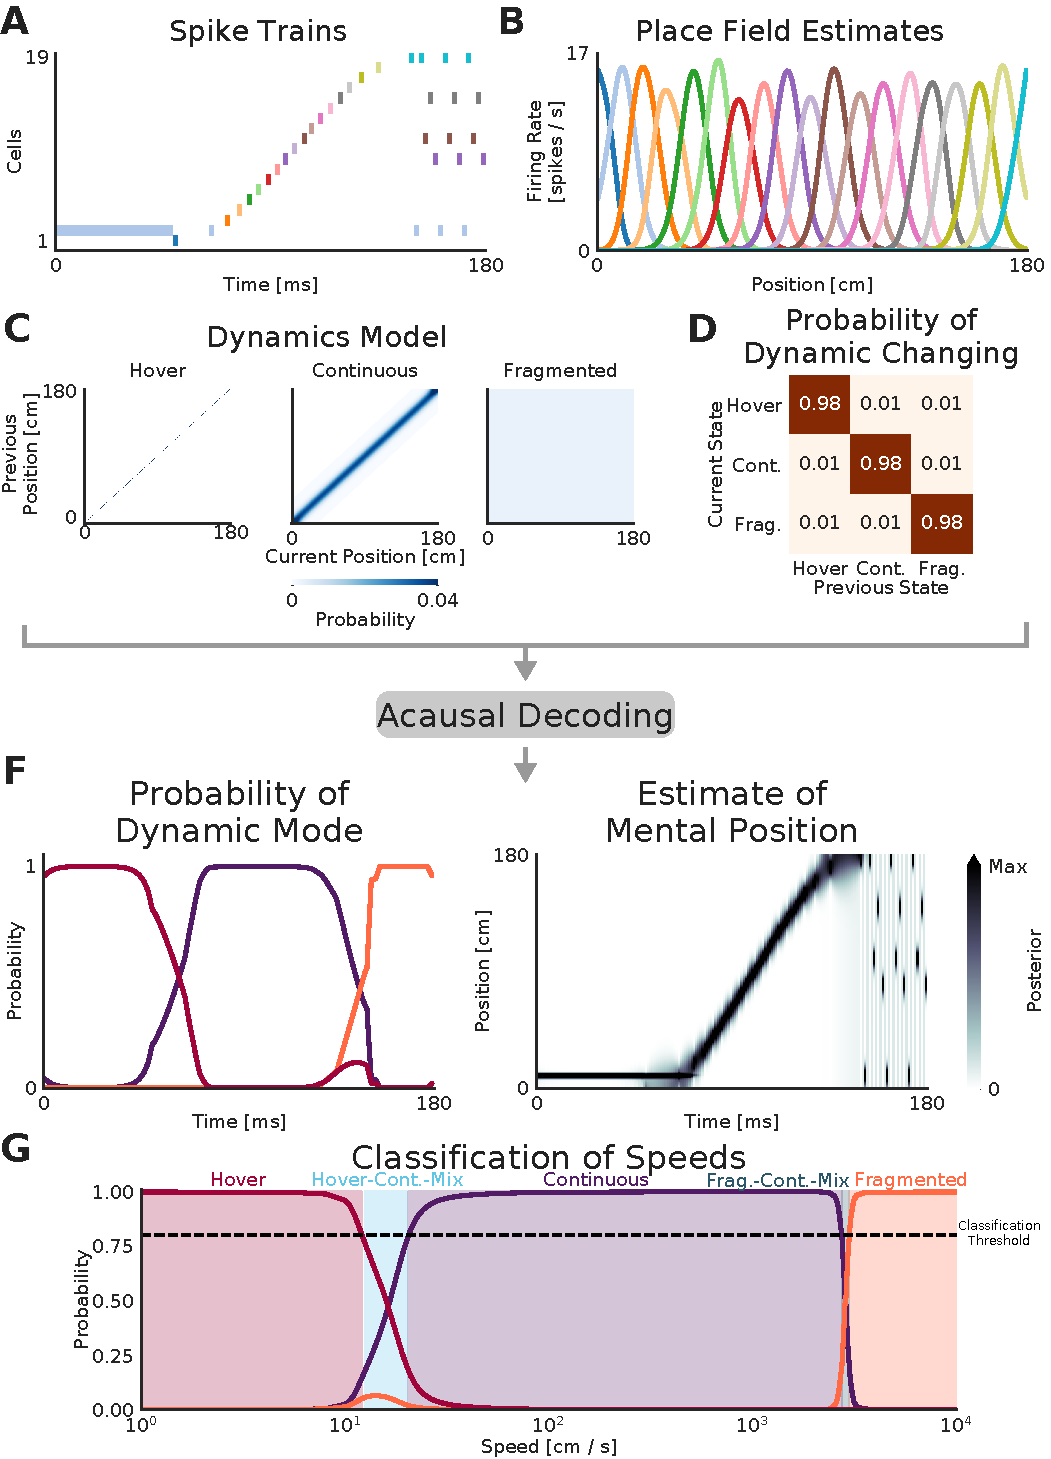
\includegraphics[width=0.80\linewidth]{figures/Figure1/Figure1_v3}
\caption{Components of the state space model and demonstration on simulated data. \textbf{(A)} 19 simulated place cells that exhibit three different sequence patterns. For the first third of time, one cell fires repeatedly, representing one stationary location. For the second third of time, the cells fire in sequence, representing a smooth continuous trajectory through space. For the last third cells fire in an incoherent pattern, representing a non-smooth fragmented trajectory through space. \textbf{(B)} Like the Bayesian Decoder, the state space model uses estimates of cells' place fields from when the animal is moving and combines them with the observed spikes in (A) to compute the likelihood of position for each time step. \textbf{(C)} This is combined with an explicit model of each dynamic state--which determines how latent position can change based on the posterior from the previous time step. In the hover state, this is modeled as the identity matrix because the position remains the same. In the continuous state, the dynamics are modeled as a Gaussian random walk, meaning the next possible position is likely to be spatially close. In the fragmented state, the dynamics are modeled as uniform, meaning the next position is equally likely to be anywhere. Note that the states displayed only reflect the within-state dynamics. \textbf{(D)} The probability of remaining in a particular state versus switching to another state. This is modeled as having a high probability of remaining in a particular state with a small probability of switching to one of the other states at each time step. \textbf{(F)} The state space model uses the components in A-D over all time to decode the joint probability of latent position and dynamic state. The joint probability can be summarized by marginalizing over latent position (left panel) to get the probability of each dynamic state over time (lines). This can also be used to get an estimate of latent position over time (right panel). \textbf{(G)} The probability of each state given a particular constant speed trajectory. Each speed corresponds to a simulated spiking sequence at that speed. The lines correspond to the average probability of that state over the sequence. Dotted line represents the 0.8 classification threshold we use to classify each range of speeds and shaded regions correspond to the classification we have given the range of speeds.
}
\label{Figure1}
\end{figure*}

\begin{figure*}%[tbhp]
\centering
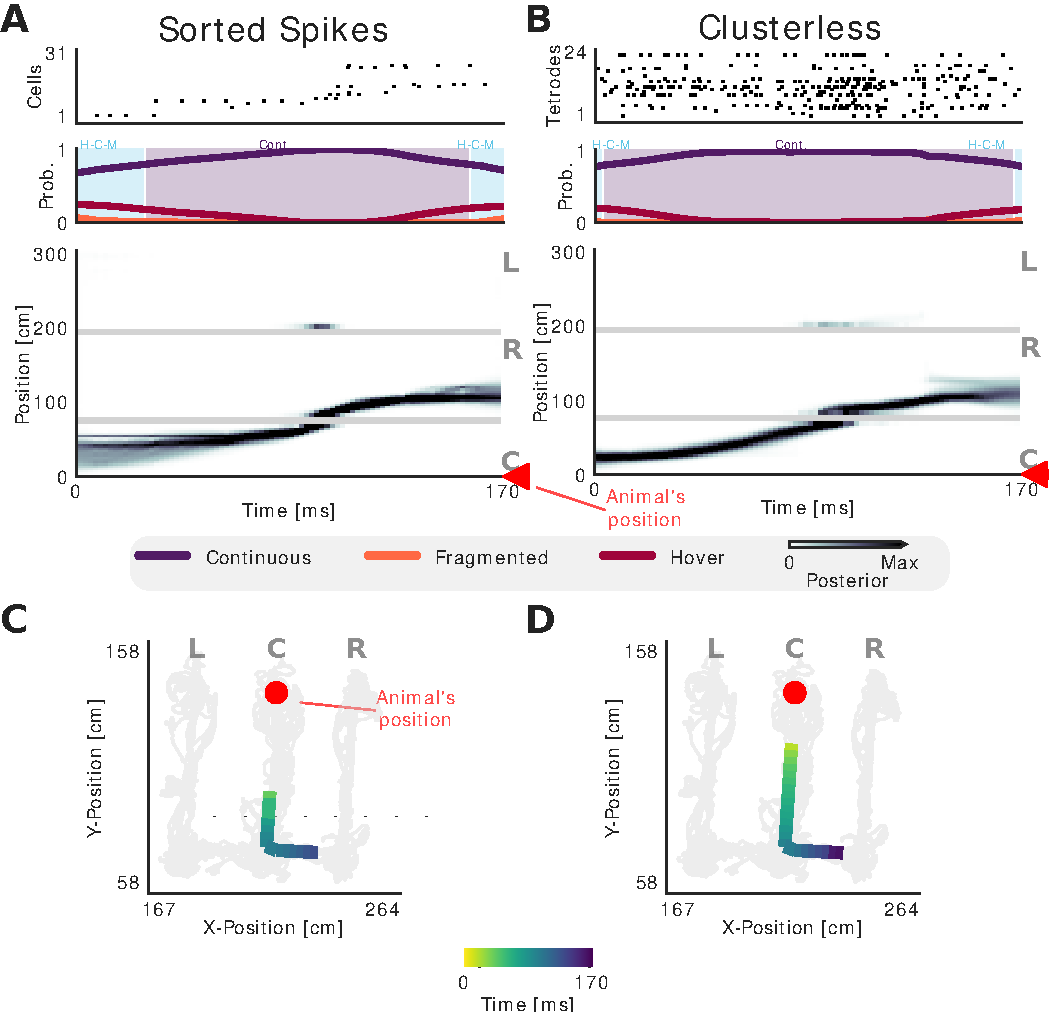
\includegraphics[width=0.80\linewidth]{figures/Figure2/Figure2_v3}
\caption{Demonstration of the state space model on real data using both sorted and clusterless spikes on the same SWR. \textbf{(A)} Decoding using sorted spikes (arranged top to bottom). In the top panel, 31 cells on a W-track ordered according to linearized position by their place field peaks. The second panel shows the probability of each dynamic over time as in Figure 1F. Shaded regions correspond to the speed classifications in Figure 1G. The third panel shows the estimated probability of latent position over the course of the SWR as it travels down the center arm toward the right arm. L, R, C correspond to the position of the left, right and center wells respectively. The animal's position is indicated by the red triangle. \textbf{(B)} Decoding using clusterless spikes. The top panel shows multiunit spiking activity from each tetrode. Other panels have the same convention as(A).  \textbf{(C)} 1D MAP estimate of the latent position in (A) projected back into 2D. Color indicates time. The animal's position is denoted by the red circle. Grey lines show the animal's 2D position over the entire epoch. L, R, and C correspond to the left, right and center well as in (A). \textbf{(D)} 1D MAP estimate of the latent position in (B) projected back into 2D. Figure conventions are the same as in (C).
}
\label{Figure2}
\end{figure*}

\begin{figure*}%[tbhp]
\centering
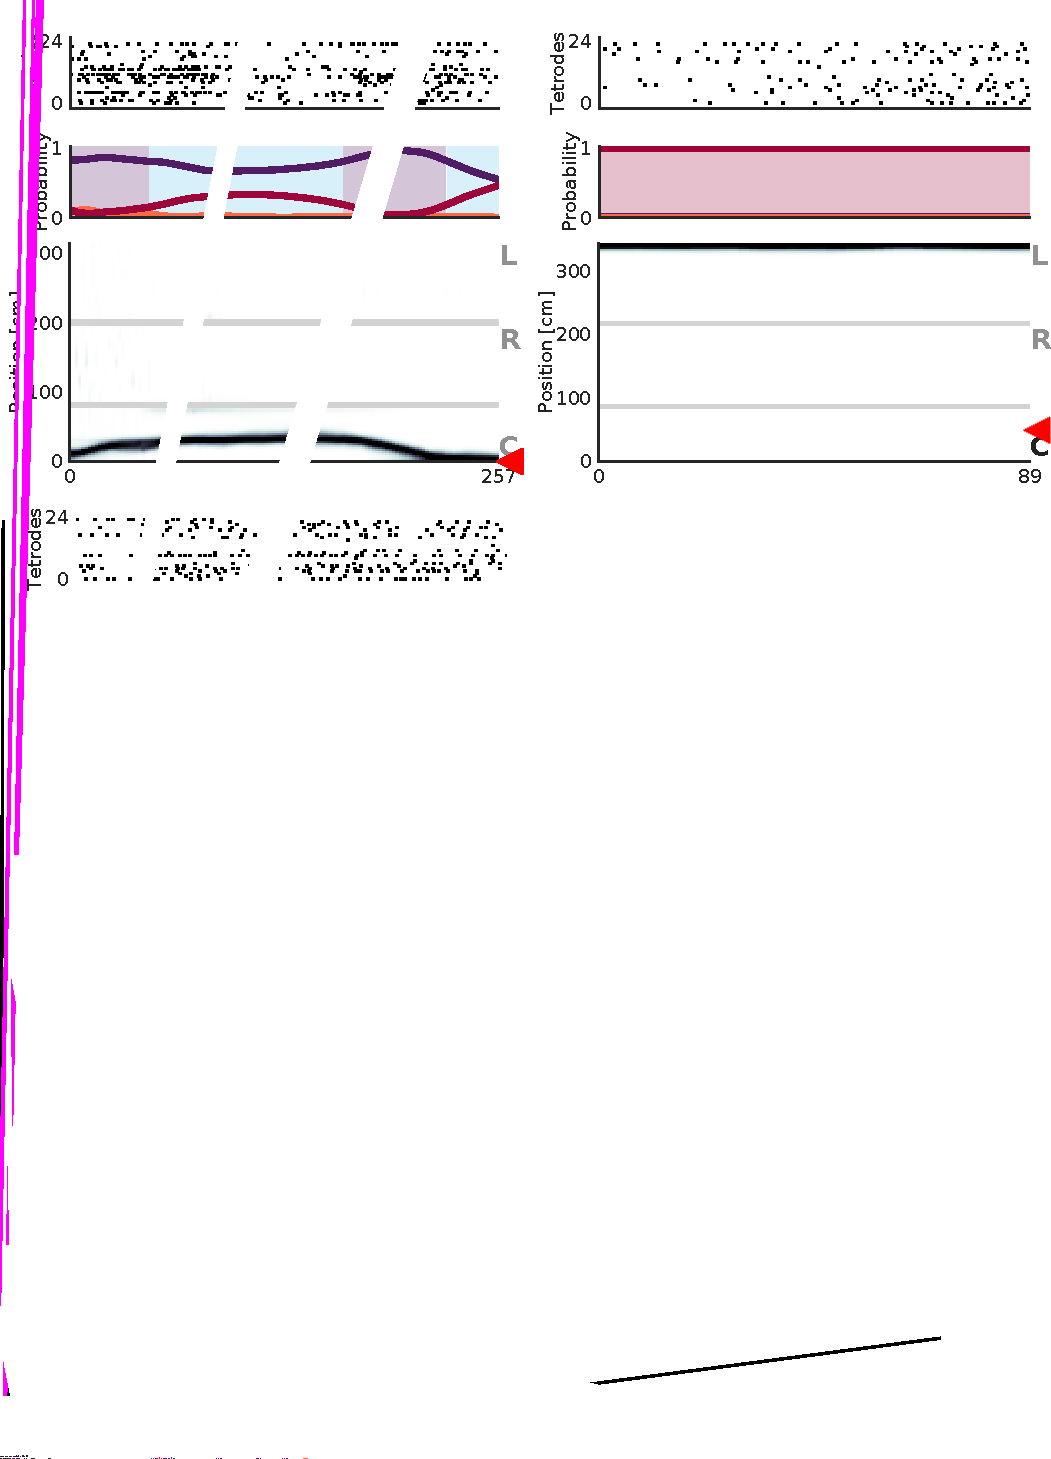
\includegraphics[width=0.80\linewidth]{figures/Figure3/Figure3_v3}
\caption{A-D. Four examples of replays that would not be well-described using the Bayesian decoder. Figure conventions are the same as in Figure 2. \textbf{(A)} A replay that starts down the center arm away from the animal's position at the center well, slows down, and returns back. \textbf{(B)} A replay that stays at the left well for the entirety of the SWR while the animal is in the center arm. \textbf{(C)} A replay that begins stationary at the left well and then jumps to the middle of the right arm and proceeds up the right arm to the right well. \textbf{(D)} A replay that begins stationary at the left well, jumps to the center arm, proceeds away from the center well, jumps to the right arm, proceeds back toward the center well, and then becomes fragmented. \textbf{(E)} Percentage of SWRs in each epoch that has some content that falls into one of the categories (Hover, Hover-Continuous-Mix, Continuous, Fragmented-Continuous-Mix, or Fragmented). \textbf{(F)} Of the classified content, the percentage of SWRs in each epoch that have some Hover, Hover-Continuous-Mix, or Continuous content. \textbf{(G)} Of the classified content, the percentage of SWR in each epoch that has some Continuous content.
}
\label{Figure3}
\end{figure*}

\begin{figure*}%[tbhp]
\centering
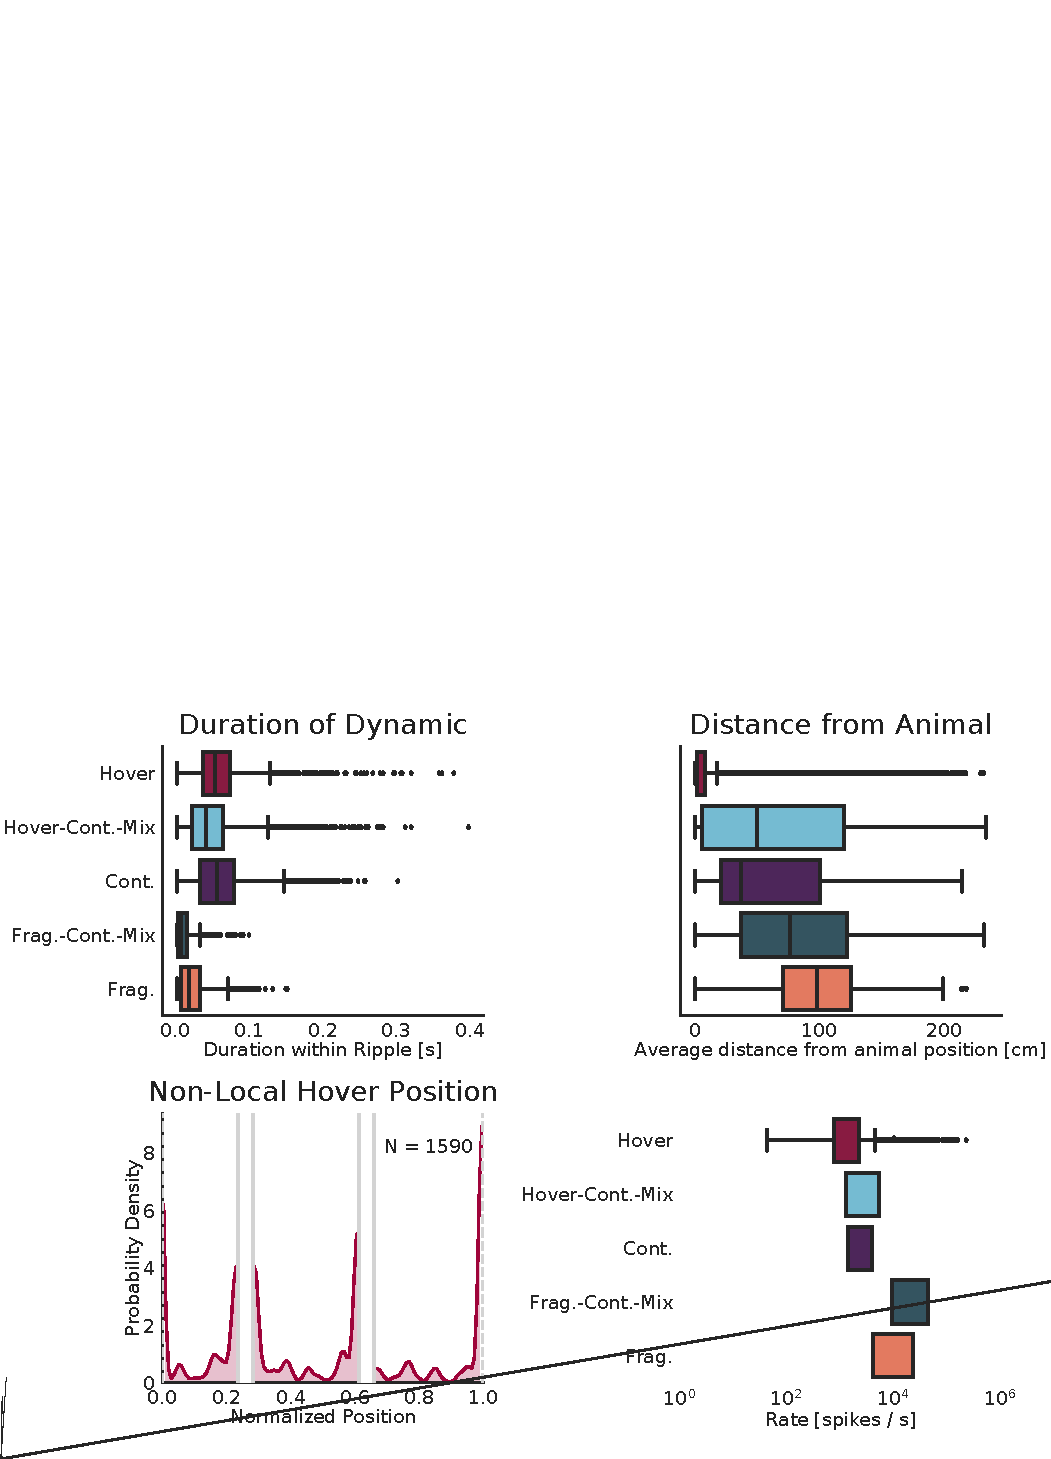
\includegraphics[width=0.80\linewidth]{figures/Figure4/Figure4_v2}
\caption{\textbf{(A)} UpSet plot of the most common combinations of dynamics within each ripple. Each row represents a possible category present in the SWR. Each column represents a set of dynamics categories, where filled-in black dots with an edge between the dots indicates that multiple categories are present in the SWR (at temporally distinct times). The sets are ordered by how often they occurred as indicated by the bar plot above each category. The total number of each category is indicated by the rotated bar plot on the left. \textbf{(B)} Box plot of the duration of each dynamic category within a ripple. \textbf{(C)} The distance of the latent position from the animal's position for each dynamic category within each ripple. \textbf{(D)} Probability density estimate 
}
\label{Figure4}
\end{figure*}


\section*{Discussion}


\begin{acknowledgements}
\end{acknowledgements}

\section*{References}
\bibliography{refs}

\onecolumn
\newpage

\section*{Methods}
\subsection*{The Model}
The 

\subsection*{Encoding - Clusterless}
In order to encode how each tetrode's unsorted spiking activity relates to position, we use a marked point process framework. For each multiunit spike during movement (defined as time periods when the running speed is greater than 4 cm/s), the associated waveform features (the marks) and position are recorded in a (n-spikes, n-features + n-position-dimensions) array. In our case, the waveform features correspond to the max amplitude observed on each tetrode wire at the time of the multiunit spike. This array is used as the training samples in a kernel density estimator during the decoding step.

\subsection*{Encoding - Sorted Spikes}
In order to encode how each cell's spiking activity relates to position (the place field), we fit a generalized linear model (GLM) with a Poisson response distribution to each cell's spiking activity during movement (defined as time periods when the running speed is greater than 4 cm/s). We estimate the parameters $\beta$, which consist of $\beta_{0}$, the average firing rate over time, and $\beta_{i}$, weights for third degree B-splines basis functions $f_{i}$ over position (or tensor products of the B-splines when position is two dimensional). B-spline basis functions are used because place field firing activity is assumed to vary smoothly over position and this prior knowledge can be exploited to reduce the total number of model parameters needed. Each basis function is spaced every 5 cm over the range of the position and zero constrained so that the change encoded by the parameters is relative to the baseline firing rate. We use a log link function to convert the linear combination of parameters to an instantaneous firing rate over time $\lambda(t)$ to ensure the rate is always positive. 

$$log(\lambda(t)) = \beta_{0} + \sum_{i} f_{i}(position)\beta_{i}$$

A small L2 penalization term $-\lambda\norm{\beta_{i}}_{2}^{2}$ used to prevent model fitting instability when spiking activity is very low. We set this to 0.5 for all cells. Fitting is done by maximizing the penalized likelihood using a Newton-Raphson algorithm.

\subsection*{Decoding - Clusterless}


\subsection*{Simulated Data}

\subsection*{Data}

\subsection*{Software and Code availability}
Python code used for analysis and generating figures in the paper is available at: \url{https://github.com/Eden-Kramer-Lab/replay_trajectory_paper}. Code for the classifier is available in a separate software repository to facilitate code reuse at: \url{https://github.com/Eden-Kramer-Lab/replay_trajectory_classification}. All code is open-source and licensed under the MIT Software License. Classifier code can be easily installed as a python package with all requisite dependencies using pip or conda. See software repositories for specific details.

\newpage

%%%%%%%%%%%%%%%%%%%%%%%%%%%%%
% Supplementary Information %
%%%%%%%%%%%%%%%%%%%%%%%%%%%%%
\beginsupplement
\captionsetup*{format=largeformat}

\begin{figure*}%[tbhp]
\centering
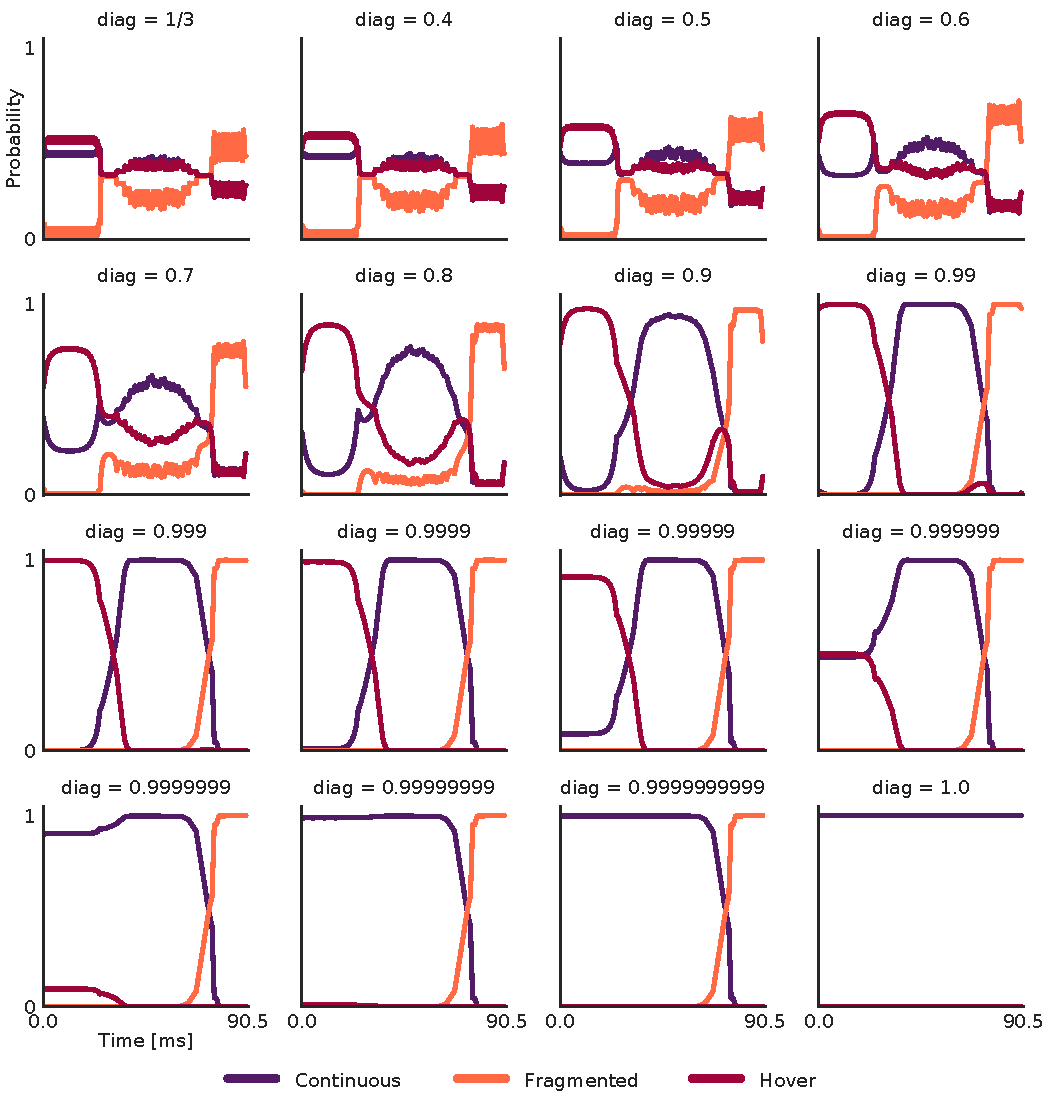
\includegraphics[width=0.80\linewidth]{figures/Figure1-supplemental1/Figure1_v1_supplemental1}
\caption{Placeholder image of Iris with a long example caption to show justification setting.}
\label{fig:Figure1-Figure supplement 1}
\end{figure*}

\begin{figure*}%[tbhp]
\centering
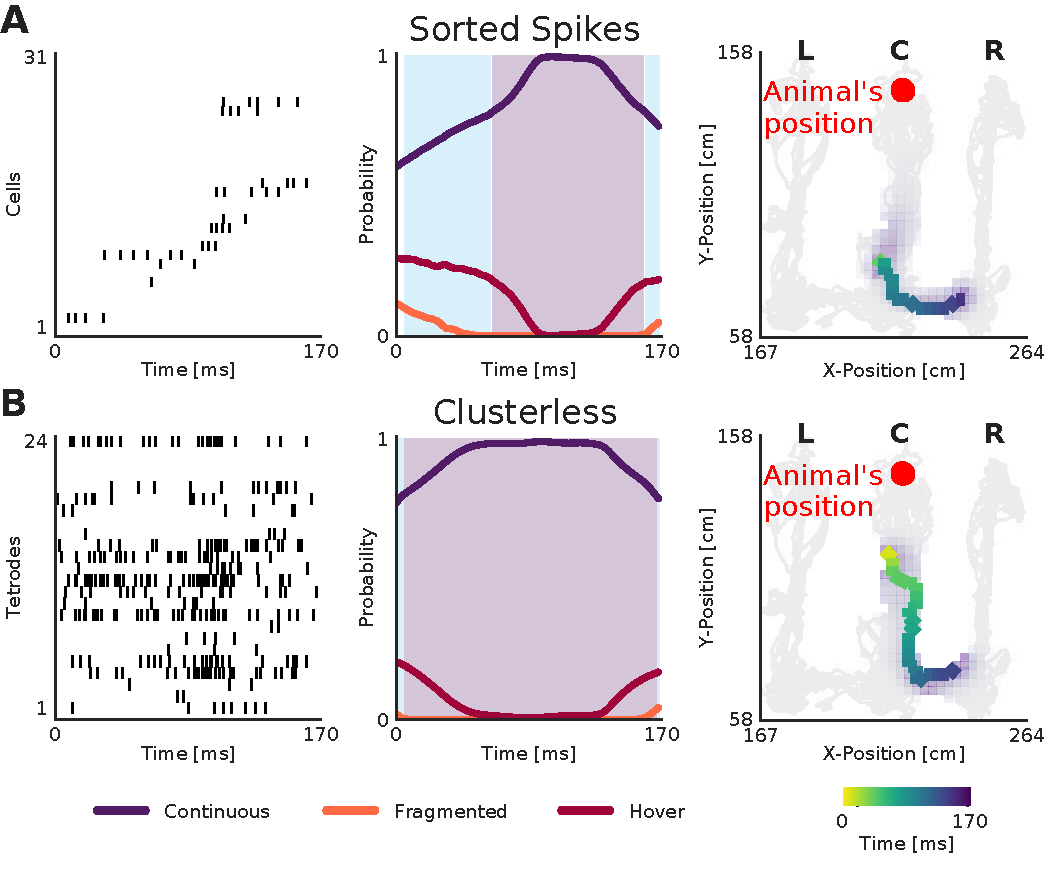
\includegraphics[width=0.80\linewidth]{figures/Figure2-supplemental1/Figure2_v2-supplemental1}
\caption{Placeholder image of Iris with a long example caption to show justification setting.}
\label{fig:Figure2-Figure supplement 1}
\end{figure*}

\begin{figure*}%[tbhp]
\centering
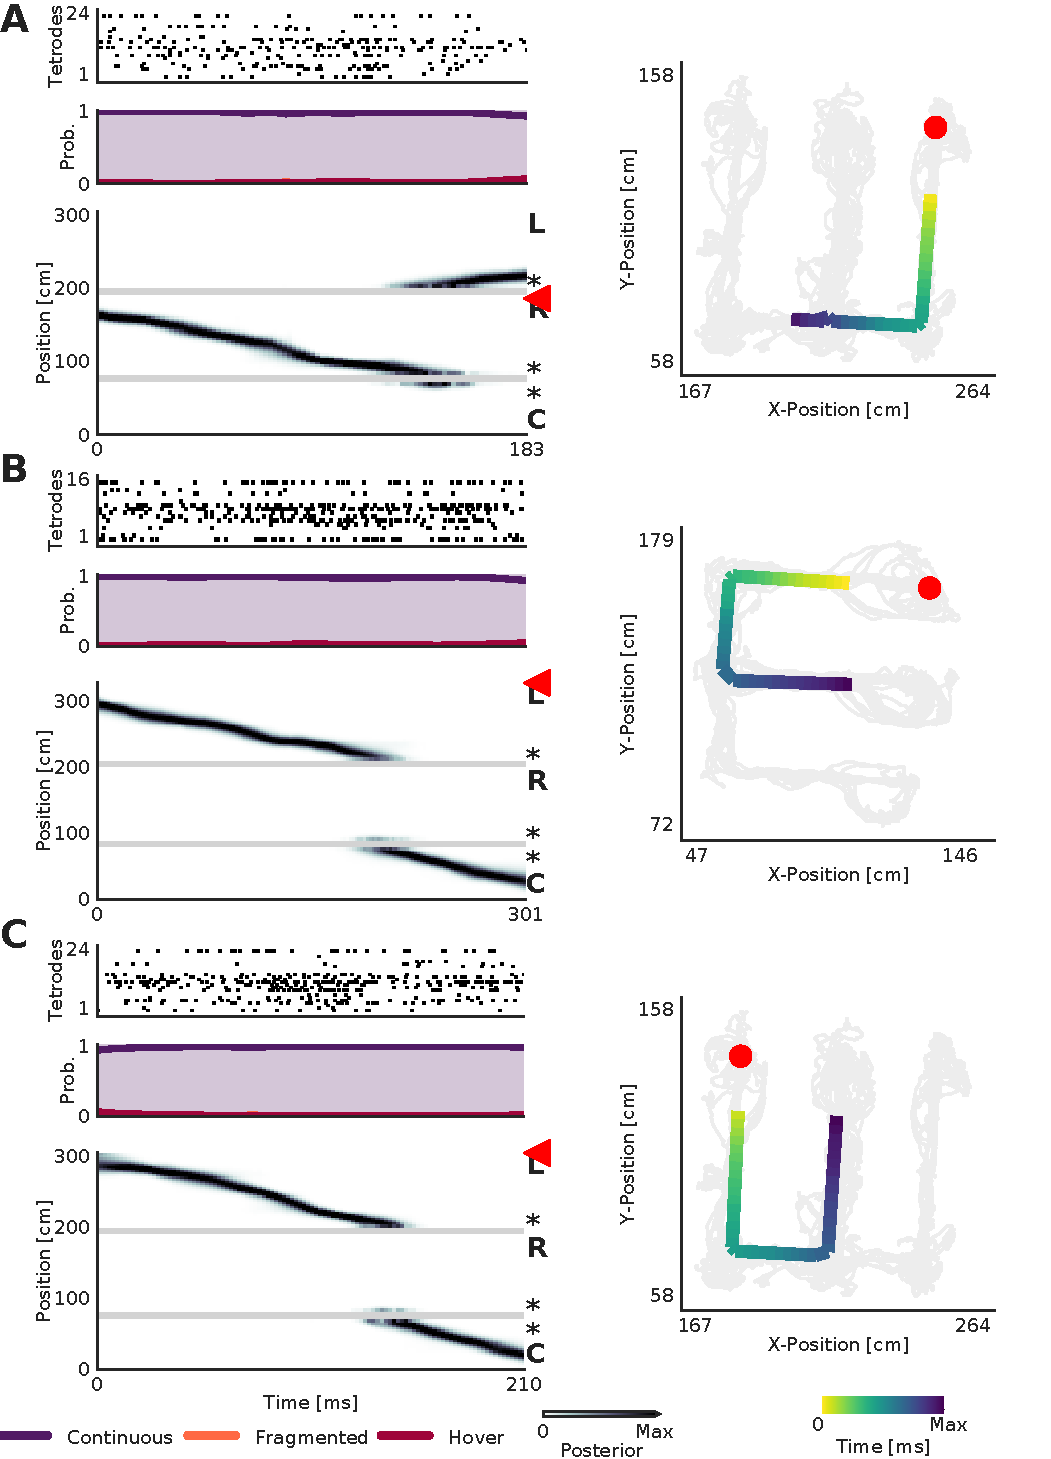
\includegraphics[width=0.80\linewidth]{figures/Figure2-supplemental2/Figure2_v2-supplemental2}
\caption{Placeholder image of Iris with a long example caption to show justification setting.}
\label{fig:Figure2-Figure supplement 2}
\end{figure*}

\begin{figure*}%[tbhp]
\centering
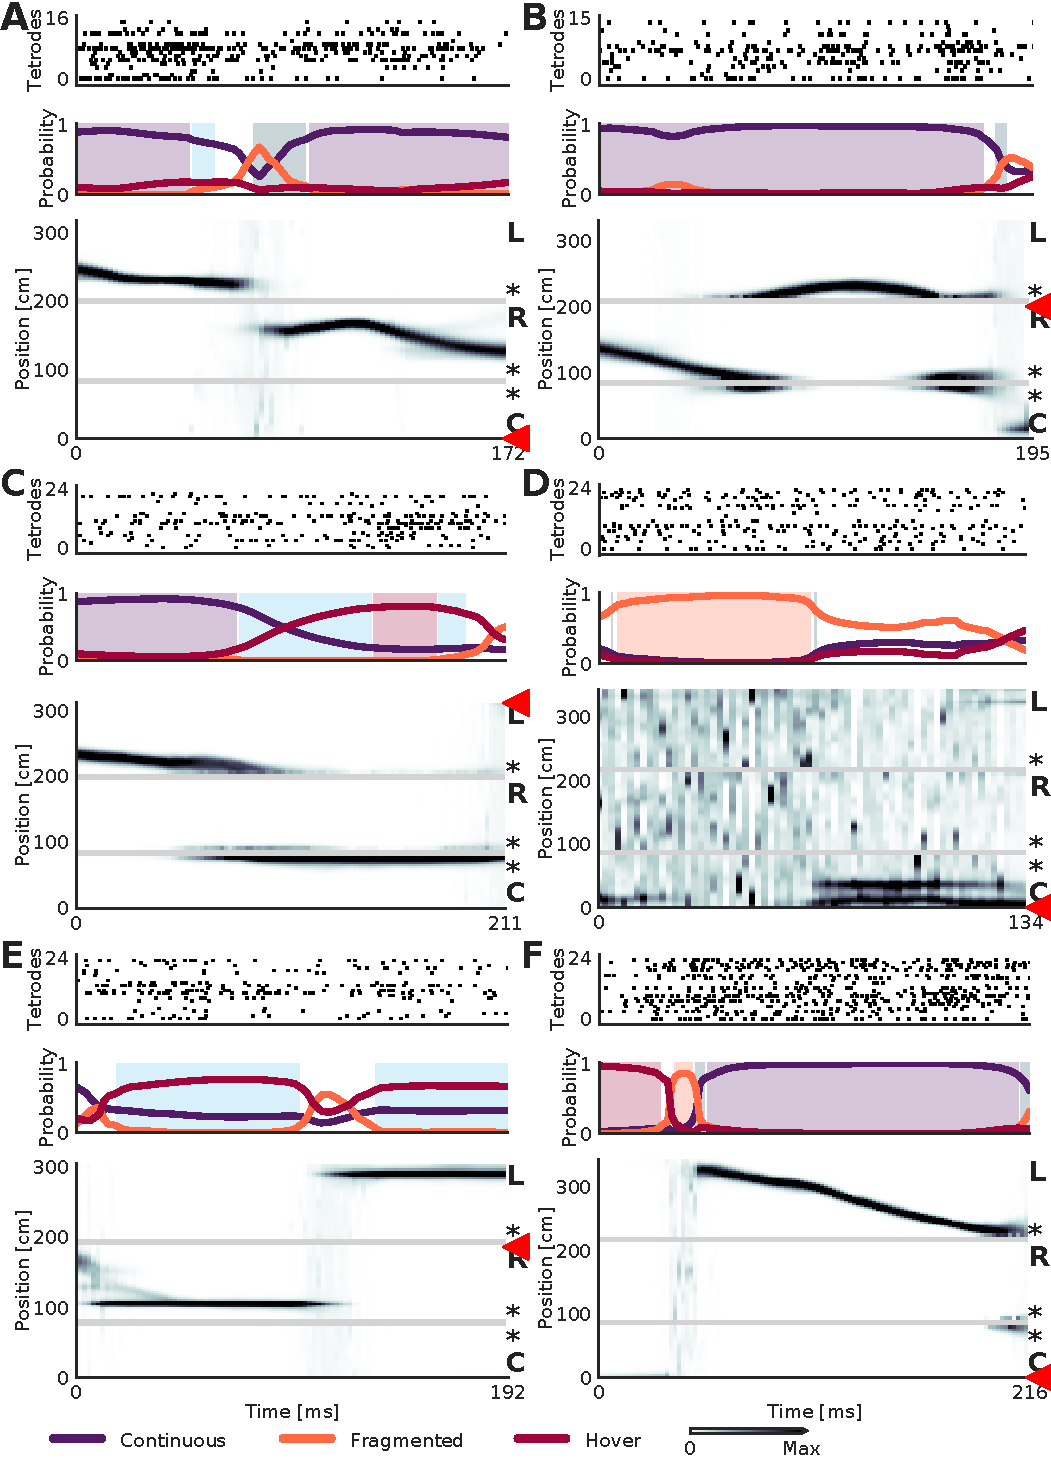
\includegraphics[width=0.80\linewidth]{figures/Figure3-supplemental1/Figure3_v2_supplemental1}
\caption{Placeholder image of Iris with a long example caption to show justification setting.}
\label{fig:Figure3-Figure supplement 1}
\end{figure*}


%TC:endignore
%the command above ignores this section for word count

\end{document}
